\documentclass[../thesis.tex]{subfiles}

\begin{document}

\subsection{Collision statistics of non-interacting droplets under two-way momentum coupling\label{sec:2way}}
In this section, 

\subsubsection{Flow statistics}

\begin{table}[!b]%---------- T A B L E ----------
\center
  \begin{tabular}{cccccccccccc}
  \hline
  $N$ & $\nu$ & $\tau_\text{K}$ & $\eta_\text{K}$ & $T_e$ & $L_f$ & $\epsilon$ & $u'$ & $R_{\lambda}$ & $k_\text{max}\eta_\text{K}$ & $\mathcal{S}$ & $\mathcal{F}$ \\\hline
  64 &  0.0070 & 0.20 & 0.0037 & 3.91 & 1.63 & 0.17 & 0.82 & 75  & 1.14 & --0.42 & 4.51 \\
  256 & 0.0011 & 0.07 & 0.0009 & 3.77 & 1.47 & 0.20 & 0.86 & 197 & 1.14 & --0.51 & 6.05 \\
  \hline
  \end{tabular}
\caption{Average particle-free flow statistics in spectral units for two different mesh resolutions.}
\label{Table2}
\end{table}%------------------------------------

As a preliminary step, we have performed simulations of turbulent flows without particles using meshes of resolutions $64^3$ and $256^3$. Averaged statistics quantifying these turbulent flows at the statistically steady state are summarized in Table~\ref{Table2}. Similar to previous parts of the discussion, the flows were enforced using the deterministic forcing scheme. The statistics of flows forced by the stochastic scheme have been published in \cite{RPAGW13}. The parameters in Table~\ref{Table2}, given in spectral units, have already been defined when discussing Table~\ref{tab:1}. In the simulations, viscosity was kept as small as possible, guaranteeing the stability of integration of the Navier--Stokes equations. This allows us to obtain flows at larger Taylor-microscale Reynolds numbers $R_{\lambda}$. The effect of the resolution parameter $k_\text{max}\eta_\text{K}$ on the collision statistics has already been discussed in \cite{RPW20}.

When conducting an investigation that requires simulations at high mesh resolutions, it is useful to estimate their computational cost, resources needed and feasibility. Here we need to perform a set of simulations with different grid sizes to address the effect of the Reynolds number on the statistical quantities of the dispersed phase. Since the simulations at a coarse resolution, i.e.\ $64^3$, do not require additional parameterizations, such as the super-droplet approach, we treat them as reference. In these simulations the side length of the computational domain is approximately 10~cm when converted to physical units. This size increases at higher mesh resolutions, also enhancing the volume of the box. To keep similar values of the droplet mass loading in the box it is necessary to trace many more droplets, which is likely to be beyond computational reach.

\subsubsection{Collision statistics}

The first set of simulations with the particles was performed on a coarse mesh, i.e.\ at resolution $64^3$, and for different mass loadings $\Phi_m$ in the range $[0, 1]$. Here 0 refers to simulations under one-way coupling and 1 represents systems in which the total mass of the droplets is equal to the mass of air in the entire domain. In all simulations we used the same physical value of the air kinematic viscosity equal to 0.17~cm$^2$/s. The energy dissipation rate (needed for rescaling units) was set to 400~cm$^2$/s$^3$. To evaluate the effect of gravity the systems were modeled considering both settling and non-settling droplets (neglecting gravitational acceleration). The results of simulations at $64^3$ are particularly important and may be used as a reference for those performed at higher resolutions since there is no need to employ the super-droplet approach. This, of course, has a positive impact on physical fidelity of the modeled statistics. Here, we analyze the kinematic properties of droplets with radii from 20 to 50~$\mu$m. For such droplets, the mechanism of collision--coalescence and in consequence their growth are strictly dependent on features of turbulent flows. The other mechanisms such as condensation or gravitational collision--coalescence (not considered here) are not as effective. We should point out that only geometric collisions without aerodynamic interactions have been considered. Hence, the particles are allowed to overlap (pass through each other), and no explicit contact collision model is implemented \citep[unlike][which relocate one particle after collisions]{ARPW21}.

\begin{figure}%----------- F I G U R E ----------
\center
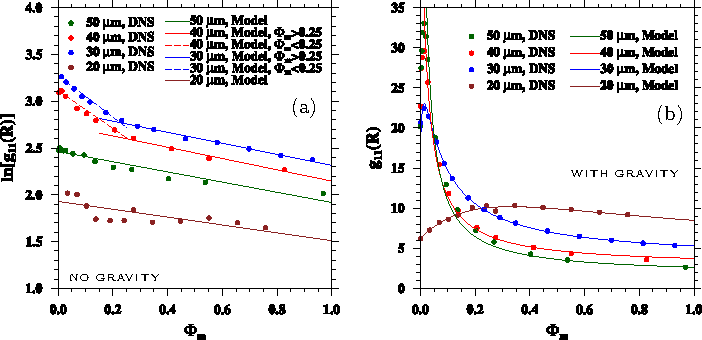
\includegraphics[width=\textwidth]{./figs/IJMF/Figure2.pdf}
\caption{The RDF of droplets computed in simulations (a) without and (b) with gravity on a grid of size 64$^3$ ($R_{\lambda}=75$).}
\label{fig1}
\end{figure}%------------------------------------

Figure~\ref{fig1}(a) shows the natural logarithm of monodisperse radial distribution function (RDF) at contact as a function of droplet mass loading in simulations without gravity. The data were computed in simulations without considering gravity. Four series of simulations were performed, each for a different droplet radius. The results of equivalent simulations with gravity are shown in Figure~\ref{fig1}(b). Note that the RDF in panel (b) is not shown in a logarithmic scale. The lines represent the best fit to the simulated data. In the first (no gravity) case, the RDF is larger for mid-inertia droplets due to their stronger clustering. For low- and high-inertia droplets clustering is weaker and pretty much linear in the entire range of considered mass loadings. This may be explained as follows. Low-inertia droplets modulate turbulent flow gently and behave like fluids elements such that the RDF stays relatively low. Increasing the number of droplets leads to a suppression of some vortex structures \citep[see][]{RPW20} which in turn results in a slight but noticeable reduction in RDF. In case of high-inertia droplets, the mechanism is different. The motion of such droplets is more decorrelated from the air flow. Therefore, modulation of turbulent field does not have a significant effect on the particle clustering and consequently on RDF.

The largest RDFs with respect to $\Phi_m$ occur for droplets at the most responsive Stokes numbers, i.e.\ when $St\approx1$. For droplets of radii 30 and 40~$\mu$m the Stokes numbers are 0.57 and 1.01, respectively. It has been established in the literature, \citep[e.g.][]{GW13}, that such particles reveal a strong tendency for clustering. Hence, the RDF reaches its maximum values. Increasing the mass loading results in a more intense damping of the smallest vortices, making the distribution of droplets more uniform. The results obtained from numerical simulations show that the slope of the logarithm of RDF (see Figure~\ref{fig1}(a)) in the range of $\Phi_m < 0.25$ is clearly larger than that for larger mass loadings. Interestingly, the RDF slope of 30 and 40~$\mu$m droplets for $\Phi_m > 0.25$ is similar to that of 50~$\mu$m droplets. The lines in Figure~\ref{fig1} have been fitted to each set of data separately. Since the observed dependency is strongly nonlinear it is difficult to develop a generic expression for RDF which will be valid for a wide range of $\Phi_m$ and droplet inertia. %In Appendix we propose a formula which fairly represents RDF for larger mass loadings and depends on the particle Stokes number.

A more complex dependency of RDF on $\Phi_m$ is found for the settling droplets. As shown in Figure~\ref{fig1}(b) there is a strongly nonlinear and non-monotonic behavior of RDF at low mass loadings. However, for $\Phi_m>0.25$ this dependency flattens out. An interpretation of this effect can be found in \cite{RPW20}. In brief, the settling droplets cause formation of vortical structures which may affect particle clustering in two different ways. For low mass loadings, the eddies make the droplet distribution less uniform, so that the RDF is visibly larger. Conversely, for larger mass loadings the enhanced swirling strength breaks up the particle clusters, therefore the system becomes more homogeneous. Consequently, the RDF is closer to unity. The exception here is the RDF of 20~$\mu$m droplets. The increase observed for low $\Phi_m$ is due to formation of new vortical structures by the settling droplets.

The development of parameterization, i.e.\ an analytical function binding the RDF and mass loading, is rather complicated. Nevertheless, a rational formula is proposed that reasonably represents the RDF in the range of $\Phi_m>0.1$ where it is mainly a function of the particle inertia. The approximating function has eleven free coefficients that were obtained by curve fitting. The resulting expression is
\begin{equation}
g_{11}(\Phi_m, St)={{{\Phi_m^2 (b_1St+b_2)+\Phi_m (b_3\exp(c_1St)+b_4) }+b_5{St^{c_2}}} \over { \Phi_m^2+\Phi_m d_1St^{c_3}+d_2{St^{c_4}}}}
\label{eq_pWG}
\end{equation}
with the coefficients listed in Table~\ref{Table3}. Interestingly, for low-inertia droplets (20~$\mu$m) the formula accurately represents the RDF even at $\Phi_m<0.1$.
\begin{table}[!b]%---------- T A B L E ----------
\center
\begin{tabular}{lccc}
\hline
Index & $b$ & $c$ & $d$ \\
\hline
1     &--1.87944 & --5.95759 & 0.01908 \\
2     &  4.63438 & --5.60405 & $1.388 \times 10^{-4}$ \\
3     &  32.5182 & --2.23761 &    \\
4     &  1.01895 & --6.84831 &     \\
5     &  $4.75907 \times 10^{-4}$ & & \\
\hline
\end{tabular}
\caption{The curve-fitting coefficients for Equation~\ref{eq_pWG}}
\label{Table3}
\end{table}%------------------------------------

\begin{figure}[h!]%----------- F I G U R E ----------
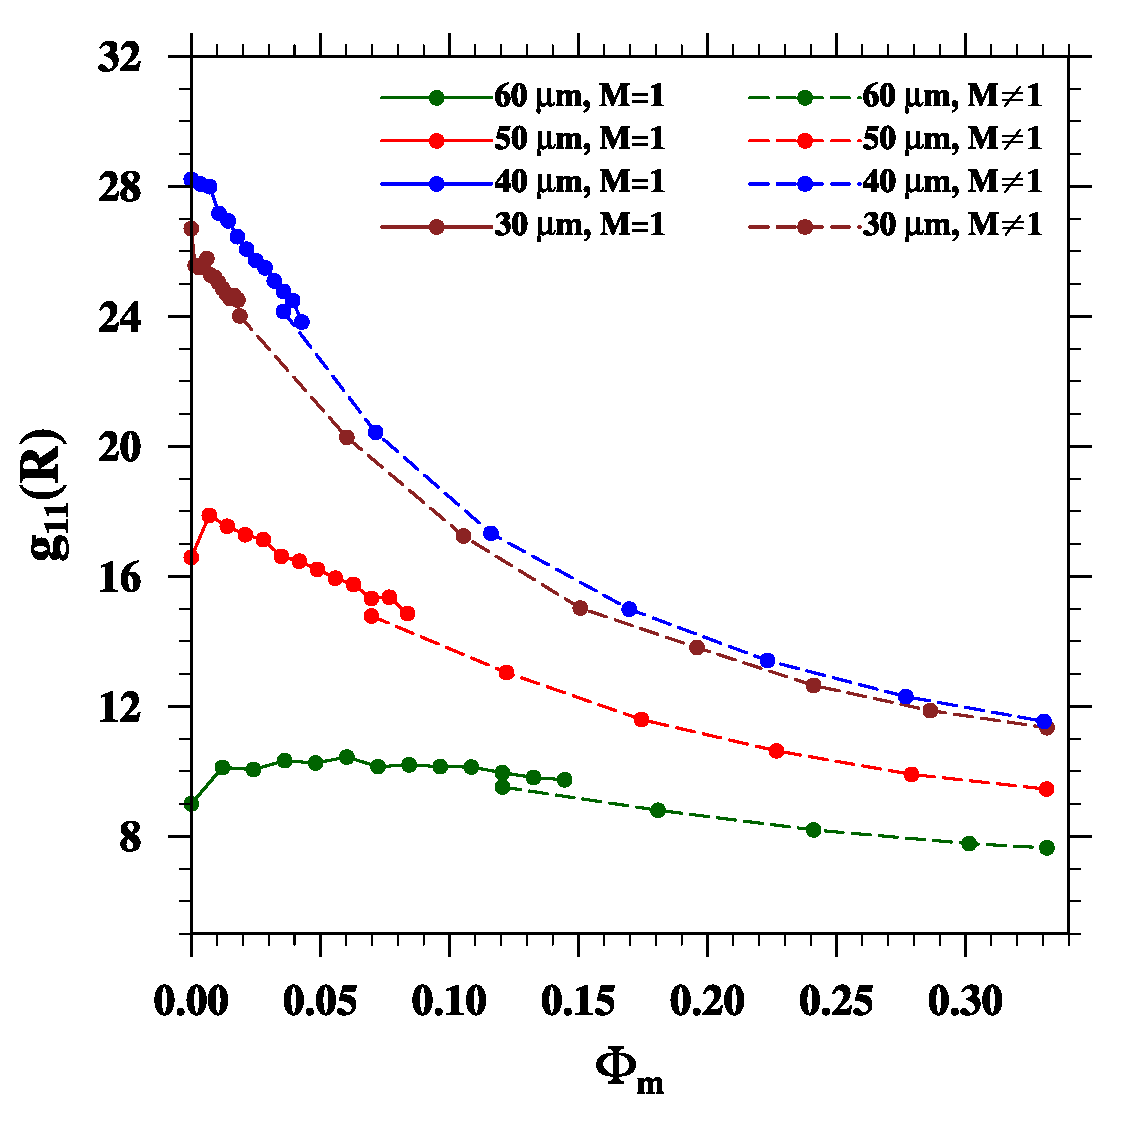
\includegraphics[width=0.5\textwidth]{./figs/IJMF/Figure3a.pdf}
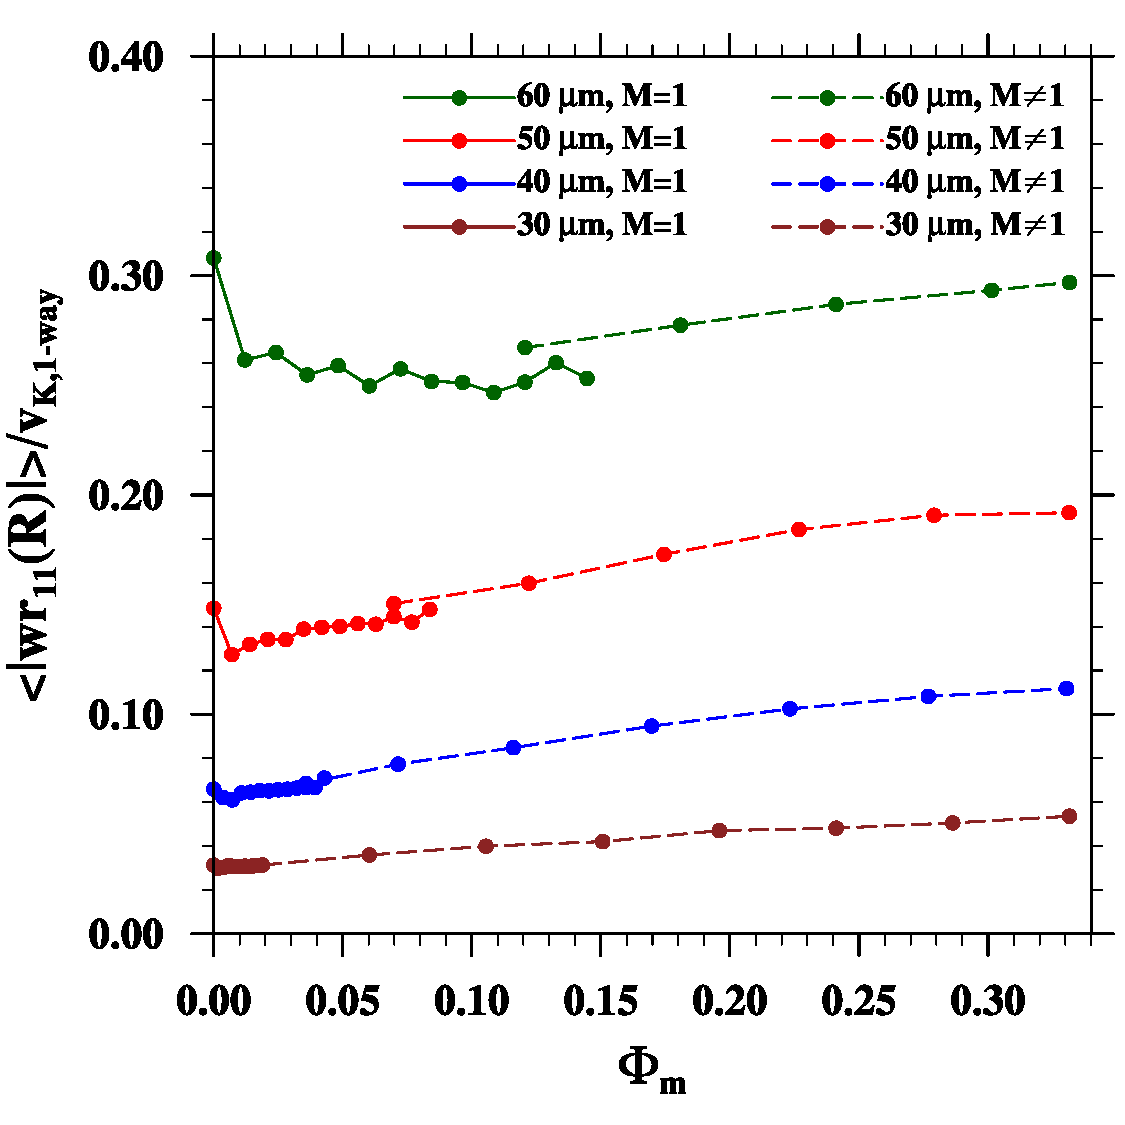
\includegraphics[width=0.5\textwidth]{./figs/IJMF/Figure3b.pdf}
\caption{The monodisperse (a) RDF and (b) normalized RRV of different sizes droplets as a function of the mass loading. Four series of simulations were performed on a grid of size $256^3$ ($R_{\lambda}=197$), neglecting gravity. Dashed lines: simulations based on simplified approach, namely, one computational particle represents $M$ real particles. The maximum value of $M~(=44)$ was used in the simulations with 30~$\mu$m droplets at $\Phi_m = 0.35$.}
\label{fig3}
\end{figure}%------------------------------------

Subsequent series of two-way coupled simulations have been performed on a mesh of higher resolution $256^3$. Due to the otherwise prohibitive cost of the simulations, the range of considered mass loadings was narrowed down to 0.35. The modeled systems were monodisperse and the influence of gravity was neglected. Here, the focus is on both kinematic collision statistics, i.e.\ the RDF and the RRV \citep[see][for the definition]{RPAGW13}. Figure~\ref{fig3} shows the statistics of nearly touching droplets, i.e.\ at a separation $r = R$, as a function of mass loading. The results obtained in simulations on the mesh $256^3$ illustrate the effect of parameterization. In the case of the RDF, we notice a slight underestimation in simulations with $M>1$, while for the RRV there is a practically smooth transition from the exact model to the parameterization for all considered droplet sizes. These results are consistent with an earlier study by \cite{RPW20}.

Another aspect concerns sensitivity of the collision statistics to $\Phi_m$. As expected, the RDF decreases with mass loading. This is a direct effect of damping the vortical structures, which are the main mechanism that enforce particle clustering. Conversely, for the RRV we observe an opposite trend. The little enhancement is due to momentum transfer from particles to the fluid. The additional momentum causes an increase in the local fluid velocity at the grid scale so that the motion of the neighboring droplets is more strongly decorrelated. As discussed, to examine the effect of having a larger $\Phi_m$, simulations with super-droplet parameterizations are necessary to reduce the computational cost.

\subsubsection{Summary}
The kinematics of inertial particles in homogeneous isotropic turbulence has been examined considering a two-way momentum coupling between the flow and particles. To address the effect of the range of turbulent scales on the dispersed phase, the simulations were performed using meshes of two different resolutions. Since the simulations with high-resolution meshes require larger mass loadings that are prohibitively expensive, we had to use a parameterization, the so-called super-droplet approach, that significantly reduces computational cost but impairs accuracy.

The effect of gravity on the statistics was also examined by performing the same simulations with and without gravity. It has been found that, for non-settling droplets, the monodisperse RDF decreases with the mass loading in all modeled cases, i.e.\ at different droplet inertia and Reynolds numbers. In other words, the spatial distribution of the particles becomes more uniform when the particle concentration increases. This is a consequence of vortical structures being damped by the motion of particles. In the presence of gravity, the RDF is non-monotonic. In the range of low mass loadings, compared to simulations under one-way momentum coupling, the RDF slightly increases with the mass loading. This amplification results from the interaction of the droplets with the vortices forced by the motion of the dispersed phase. For larger mass loadings, the RDF systematically decreases, and this is a consequence of stronger swirling strength which makes the system more uniform and homogeneous. We also noticed that the results are sensitive to the parameterization (super-droplet approach), particularly to the $M$ parameter. Thus, the results obtained via a larger $M$, at higher $R_{\lambda}$ using higher mesh resolutions, can only be interpreted qualitatively.

Regarding the relative motion of the droplets, we observed a significant enhancement of RRV by increasing the mass loading. This is due to the momentum transfer from droplets to the fluid, which causes a more effective decorrelation in their motion. Results from simulations on higher mesh resolutions reveal a huge increase of RRV at larger mass loadings. Overall, the RRV is more sensitive to the $M$ parameter than the RDF.

%\bibliographystyle{refs}
%\bibliography{refs}
\newpage
\end{document}
